\documentclass[10pt,twocolumn]{article}

% ---------- Packages ----------
\usepackage[utf8]{inputenc}
\usepackage[T1]{fontenc}
\usepackage[margin=2.1cm]{geometry}
\usepackage{graphicx}
\usepackage{booktabs}
\usepackage{amsmath}
\usepackage{amssymb}
\usepackage{float}
\usepackage{caption}
\usepackage{hyperref}
\usepackage{xcolor}
\usepackage{tikz}
\usetikzlibrary{positioning,arrows.meta}
\hypersetup{colorlinks=true,linkcolor=blue!55!black,citecolor=blue!55!black,urlcolor=blue!55!black}
\captionsetup{font=small,labelfont=bf}

% ---------- Title ----------
\title{\vspace{-1.2em}Does Removing Non-Anatomical Artifacts from Chest X-Rays
Improve Pneumonia Classification?}
\author{Aleksandr Sorokin \and Viggo Beck \and Sebastian Drumm \and Hero Engelund\\[2pt]
\small Applied Artificial Intelligence --- Exam Project}
\date{\small \today}

\begin{document}
\maketitle

% =====================================================================
\begin{abstract}
\noindent
Chest X-rays carry burned-in orientation markers (the letters \emph{R}/\emph{L})
and other non-anatomical text that a convolutional neural network (CNN) might
exploit as a shortcut instead of learning genuine pathology. We ask whether
removing these artifacts improves pneumonia classification. Following Nunamaker
et~al.'s multi-methodological process, we built a reproducible PyTorch pipeline
on the Kaggle \emph{Chest X-Ray Images (Pneumonia)} dataset (5{,}856 images),
re-split 80/10/10, and trained a custom three-block CNN. We then ran a
\emph{locked} experiment: one model trained on the original images and one on a
copy in which bright marker artifacts were detected with OpenCV and inpainted,
with every other factor held identical. The cleaned dataset produced essentially
no change in held-out test performance (Youden's J $-0.0023$, AUC $-0.0001$,
accuracy $-0.0017$). We conclude that, for this dataset and architecture,
removing the markers neither helps nor hurts: the classifier's decisions are
already driven by the lung fields rather than the markers.
\end{abstract}

% =====================================================================
\section{Introduction}
\label{sec:intro}
Pneumonia is a leading cause of death worldwide, and the chest X-ray remains the
most common first-line imaging examination for diagnosing it. Deep convolutional
neural networks now match or exceed clinicians on several chest-X-ray tasks
\cite{rajpurkar2017chexnet}, which makes them attractive as triage tools.

A recurring danger in medical imaging, however, is \emph{shortcut learning}: a
model reaches high accuracy by latching onto spurious correlations rather than
the intended signal \cite{geirhos2020shortcut}. Chest radiographs are a textbook
case. Zech et~al.\ showed that CNNs can key on hospital-specific tokens burned
into the image and fail to generalise across institutions \cite{zech2018confound},
and DeGrave et~al.\ found that COVID-19 X-ray classifiers frequently relied on
laterality markers, text and image edges instead of lung pathology
\cite{degrave2021shortcut}. Our dataset contains exactly such artifacts: most
films carry a bright \emph{R} (or \emph{L}) orientation marker and occasional
technician text near the border (Figure~\ref{fig:samples}).

This motivates a concrete, testable question: if these non-anatomical artifacts
were removed, would a pneumonia classifier perform better? A positive answer
would suggest the model is partly cheating; a negative answer would provide
evidence that the markers are not driving its decisions. We investigate this with
a controlled, reproducible two-dataset experiment.

% =====================================================================
\section{Research Question}
\label{sec:rq}
We phrase one overall question with two supporting sub-questions.

\begin{itemize}
  \item[\textbf{Q1}] Does removing non-anatomical artifacts (e.g.\ the orientation
  marker \emph{R}) from chest X-rays improve pneumonia classification
  performance?
  \item[\textbf{Q1.1}] How can the artifacts be detected and removed reliably and
  time-efficiently, without damaging anatomy?
  \item[\textbf{Q1.2}] How should the strong class imbalance between
  \textsc{normal} and \textsc{pneumonia} images be handled so that it does not
  confound the comparison?
\end{itemize}

\noindent
To answer Q1 we keep \emph{every} factor constant between two training runs and
change only one thing --- whether the input images still contain the artifacts ---
so that any difference in test performance is attributable to the cleaning alone.

% =====================================================================
\section{Methods}
\label{sec:methods}
We follow Nunamaker et~al.'s multi-methodological systems-development process
\cite{nunamaker1990}, iterating between observation, systems development and
experimentation. Every step from data import to evaluation is scripted so the
results are transparent and reproducible; all random number generators (Python,
NumPy and PyTorch, CPU and CUDA) are seeded with a fixed value.

\subsection{Data and splitting}
\label{sec:data}
We use the Kaggle \emph{Chest X-Ray Images (Pneumonia)} dataset
\cite{kermany2018,kagglecxr}, comprising 5{,}856 paediatric frontal chest
radiographs labelled \textsc{normal} or \textsc{pneumonia}. The original Kaggle
partition has a very small validation set (16 images), so we merge all images and
re-split them \emph{by file} into 80\,\%/10\,\%/10\,\% train/validation/test
partitions with a fixed seed. The same split membership is reused for both the
original and the cleaned dataset so the comparison is image-for-image identical
(Section~\ref{sec:locked}).

\subsection{Preprocessing}
\label{sec:preproc}
Images are converted to single-channel grayscale, padded to a square (to avoid
distortion), and resized to $224\times224$ px --- the standard input size for this
family of models \cite{he2016resnet}. Pixel values are normalised to a mean and
standard deviation of $0.5$. During training only, we apply light augmentation
(rotation $\pm7^{\circ}$, translation $\pm3\,\%$, zoom $\pm3\,\%$); augmentation
is a standard regulariser that improves generalisation on limited medical data
\cite{shorten2019augment}. Validation and test images receive no augmentation.

\subsection{Class imbalance}
\label{sec:imbalance}
The dataset is imbalanced (73\,\% \textsc{pneumonia}, 27\,\% \textsc{normal}),
which can bias a classifier toward the majority class
\cite{he2009imbalanced,krawczyk2016imbalanced}. We address this with a
\texttt{WeightedRandomSampler} that draws minority-class images more often, so
each training batch is approximately class-balanced. The sampler is applied only
to the \emph{training} loader; validation and test sets keep their natural
distribution so reported metrics reflect realistic prevalence.

\subsection{Model architecture}
\label{sec:model}
We use a custom three-block CNN (Figure~\ref{fig:arch}). Each block is a
$3\times3$ convolution followed by batch normalisation \cite{ioffe2015batchnorm},
a ReLU activation and $2\times2$ max-pooling; the channel width grows
$1\!\to\!32\!\to\!64\!\to\!128$. The resulting $128\times28\times28$ feature map
is flattened into a fully connected classifier with a 256-unit hidden layer,
dropout \cite{srivastava2014dropout} and a two-way output. The design follows the
classic convolution--pooling--dense template established for image classification
\cite{lecun1998gradient,krizhevsky2012imagenet} ($\approx$25.8\,M parameters).

\begin{figure}[t]
\centering
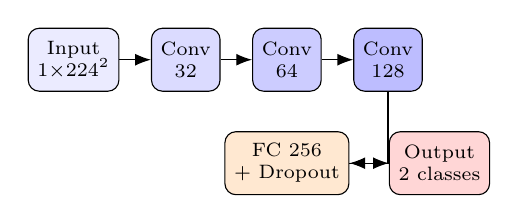
\begin{tikzpicture}[
  font=\scriptsize,
  block/.style={draw,rounded corners,minimum height=8mm,minimum width=8mm,align=center,fill=blue!8},
  arr/.style={-{Latex[length=2mm]}}]
  \node[block] (in) {Input\\$1{\times}224^2$};
  \node[block,right=4mm of in,fill=blue!14] (c1) {Conv\\32};
  \node[block,right=4mm of c1,fill=blue!20] (c2) {Conv\\64};
  \node[block,right=4mm of c2,fill=blue!26] (c3) {Conv\\128};
  \node[block,below=5mm of c2,fill=orange!18] (fc) {FC 256\\+ Dropout};
  \node[block,right=5mm of fc,fill=red!16] (out) {Output\\2 classes};
  \draw[arr] (in)--(c1); \draw[arr] (c1)--(c2); \draw[arr] (c2)--(c3);
  \draw[arr] (c3.south)|-(fc.east);
  \draw[arr] (fc)--(out);
\end{tikzpicture}
\caption{Three-block CNN. Each Conv block = $3{\times}3$ convolution +
batch norm + ReLU + $2{\times}2$ max-pool; the flattened features feed a dropout
classifier.}
\label{fig:arch}
\end{figure}

\subsection{Artifact detection and removal}
\label{sec:cleaning}
Orientation markers and technician text are bright, small, near-white blobs that
sit on a dark background close to the image border, away from the lung fields. We
detect them with OpenCV \cite{bradski2000opencv} using three independent tests on
the connected components of the brightest pixels: \emph{(i)} location --- the
blob's centroid lies in a left, right or top edge band (the bottom is excluded,
where the diaphragm and film strips appear); \emph{(ii)} shape --- a letter-like
size, aspect ratio and solidity; and \emph{(iii)} isolation --- a dark ring of
surrounding pixels, which distinguishes a marker from bright anatomy (ribs,
clavicles) that is connected to other bright tissue. Detected regions are dilated
and filled with Telea inpainting \cite{telea2004inpaint}, which reconstructs the
masked area from neighbouring pixels so no hard edge is left behind. The procedure
is scripted (\texttt{create\_cleaned\_dataset.py}) to write a second dataset with
an identical folder structure.

\subsection{Locked two-dataset experiment}
\label{sec:locked}
To answer Q1 we train two fresh models --- one on the original images, one on the
cleaned images --- while \emph{locking} the architecture, hyperparameters, split
membership, preprocessing, sampler logic, batch size and threshold-selection
method. The only variable is the dataset path, so any performance difference is
caused by artifact removal alone.

\subsection{Hyperparameter search}
\label{sec:search}
Before the locked comparison we tune the baseline with a 20-trial random search
\cite{bergstra2012random} over learning rate (log-uniform $[10^{-5},10^{-3}]$),
dropout ($[0.2,0.6]$), weight decay (log-uniform $[10^{-5},10^{-2}]$) and batch
size $\{16,32,64\}$, optimising with AdamW and a \texttt{ReduceLROnPlateau}
schedule. Trial~1 is the default configuration so the search directly answers
``did tuning beat the default?''.

\subsection{Evaluation}
\label{sec:eval}
Because missing a true pneumonia case is costly, accuracy alone is inadequate; we
report sensitivity (recall), specificity, precision, the area under the ROC curve
(AUC), and Youden's J statistic $J=\text{sensitivity}+\text{specificity}-1$
\cite{youden1950}. The decision threshold for each model is selected on the
\emph{validation} set (the point that maximises $J$) and then applied once to the
held-out test set, which is touched only for the final evaluation.

% =====================================================================
\section{Analysis}
\label{sec:analysis}
\subsection{Data observation}
The re-split data contains 4{,}684 training, 585 validation and 587 test images.
The class imbalance is clear (Figure~\ref{fig:classdist}), confirming the need for
the weighted sampler of Section~\ref{sec:imbalance}. Sample images
(Figure~\ref{fig:samples}) reveal the orientation markers and confirm the visual
difference between the classes.

\begin{figure}[t]
\centering
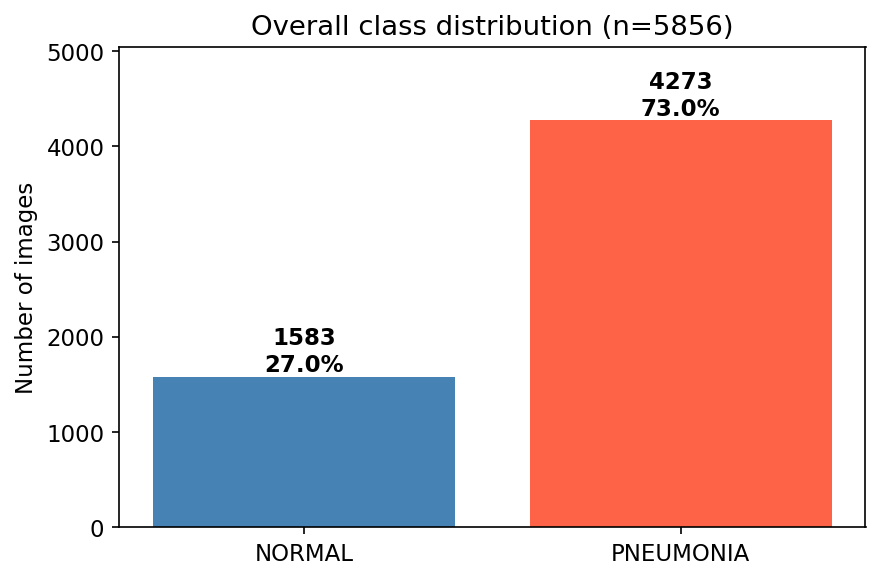
\includegraphics[width=0.86\linewidth]{figs/fig_class_dist.png}
\caption{Overall class distribution across the merged dataset. \textsc{pneumonia}
images outnumber \textsc{normal} images roughly $2.7{:}1$.}
\label{fig:classdist}
\end{figure}

\begin{figure}[t]
\centering
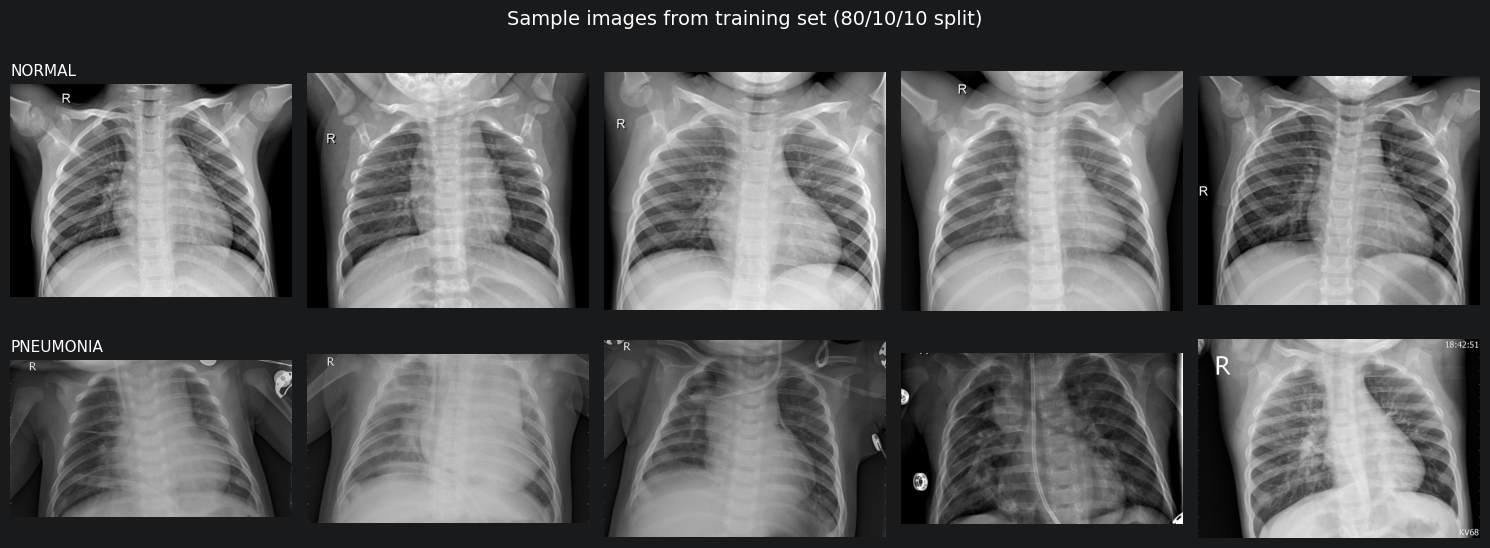
\includegraphics[width=\linewidth]{figs/fig_samples.png}
\caption{Sample training images (top: \textsc{normal}, bottom:
\textsc{pneumonia}). Bright orientation markers are visible near the borders.}
\label{fig:samples}
\end{figure}

\subsection{Artifact removal}
Applying the detector of Section~\ref{sec:cleaning} localises the bright border
markers and inpaints them cleanly while leaving the lung fields untouched
(Figure~\ref{fig:cleaning}). Visual inspection across many images confirms that
the three-test rule rarely fires on anatomy, satisfying sub-question Q1.1.

\begin{figure}[t]
\centering
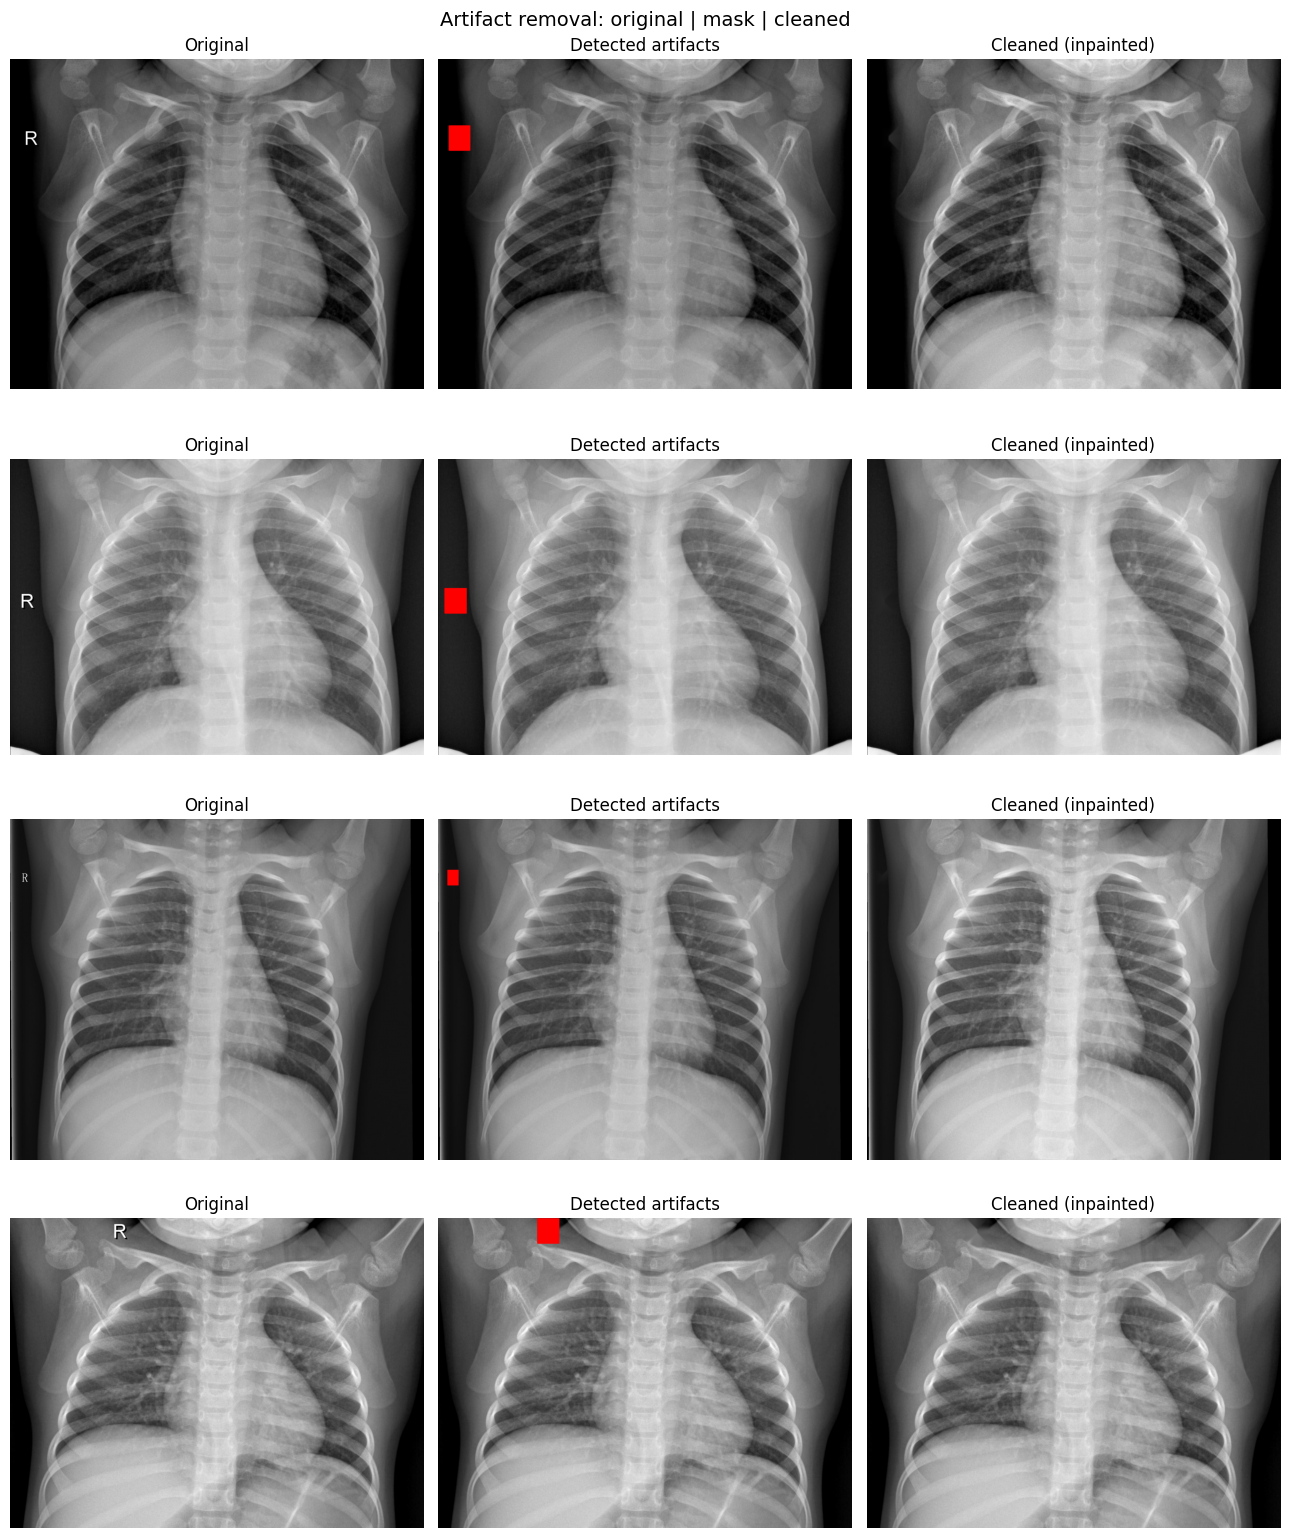
\includegraphics[width=\linewidth]{figs/fig_artifact_removal.png}
\caption{Artifact removal. Left: original. Middle: detected marker region (red).
Right: image after Telea inpainting. The \emph{R} markers are removed without
disturbing the lungs.}
\label{fig:cleaning}
\end{figure}

\subsection{Hyperparameter search}
The random search (Section~\ref{sec:search}) explored 20 configurations. The best
trial improved validation Youden's J over the default by $+0.021$
(Table~\ref{tab:search}), confirming the default configuration was already near a
good operating point; the tuned and default models are therefore both reasonable
baselines for the locked comparison.

\begin{table}[t]
\centering
\caption{Top random-search trials, ranked by validation Youden's J (the default
configuration is included for reference).}
\label{tab:search}
\small
\begin{tabular}{lccccc}
\toprule
Trial & lr & dropout & wd & Val $J$ & Val AUC\\
\midrule
random-3 & 1.5e\textnormal{-}5 & 0.37 & 1.2e\textnormal{-}5 & \textbf{0.9065} & 0.9851\\
random-1 & 1.9e\textnormal{-}4 & 0.21 & 6.7e\textnormal{-}5 & 0.9002 & 0.9870\\
random-5 & 2.0e\textnormal{-}4 & 0.42 & 4.6e\textnormal{-}5 & 0.9002 & 0.9826\\
default  & 1.0e\textnormal{-}4 & 0.40 & 0.0 & 0.8852 & 0.9857\\
\bottomrule
\end{tabular}
\end{table}

\subsection{Original vs.\ cleaned}
We then ran the locked experiment of Section~\ref{sec:locked}. Both models were
trained from scratch under identical settings and evaluated on the same held-out
test set with validation-selected thresholds. The test confusion matrices
(Figure~\ref{fig:confusion}) and the metric comparison
(Figure~\ref{fig:comparison}, Table~\ref{tab:results}) are reported in
Section~\ref{sec:findings}.

% =====================================================================
\section{Findings}
\label{sec:findings}
On the held-out test set the original-data model achieved a Youden's J of
$0.8226$ (sensitivity $0.8855$, specificity $0.9371$, accuracy $0.8995$, AUC
$0.9734$). The model trained on the cleaned data achieved a Youden's J of
$0.8203$ (sensitivity $0.8832$, specificity $0.9371$, accuracy $0.8978$, AUC
$0.9733$). The differences (cleaned minus original) are $-0.0023$ in Youden's J,
$-0.0023$ in sensitivity, $0.0000$ in specificity, $-0.0017$ in accuracy and
$-0.0001$ in AUC (Table~\ref{tab:results}).

The confusion matrices (Figure~\ref{fig:confusion}) differ by a single
case: the cleaned model classifies one additional \textsc{pneumonia} image as
\textsc{normal} (a false negative). All other cells are identical. The ROC-level
ranking, summarised by AUC, is unchanged to three decimal places.

\begin{table}[t]
\centering
\caption{Held-out test performance for the locked two-dataset experiment.
$\Delta$ is cleaned minus original.}
\label{tab:results}
\small
\begin{tabular}{lccc}
\toprule
Metric & Original & Cleaned & $\Delta$\\
\midrule
Youden's J  & 0.8226 & 0.8203 & $-0.0023$\\
Sensitivity & 0.8855 & 0.8832 & $-0.0023$\\
Specificity & 0.9371 & 0.9371 & $\phantom{-}0.0000$\\
Accuracy    & 0.8995 & 0.8978 & $-0.0017$\\
AUC         & 0.9734 & 0.9733 & $-0.0001$\\
\bottomrule
\end{tabular}
\end{table}

\begin{figure}[t]
\centering
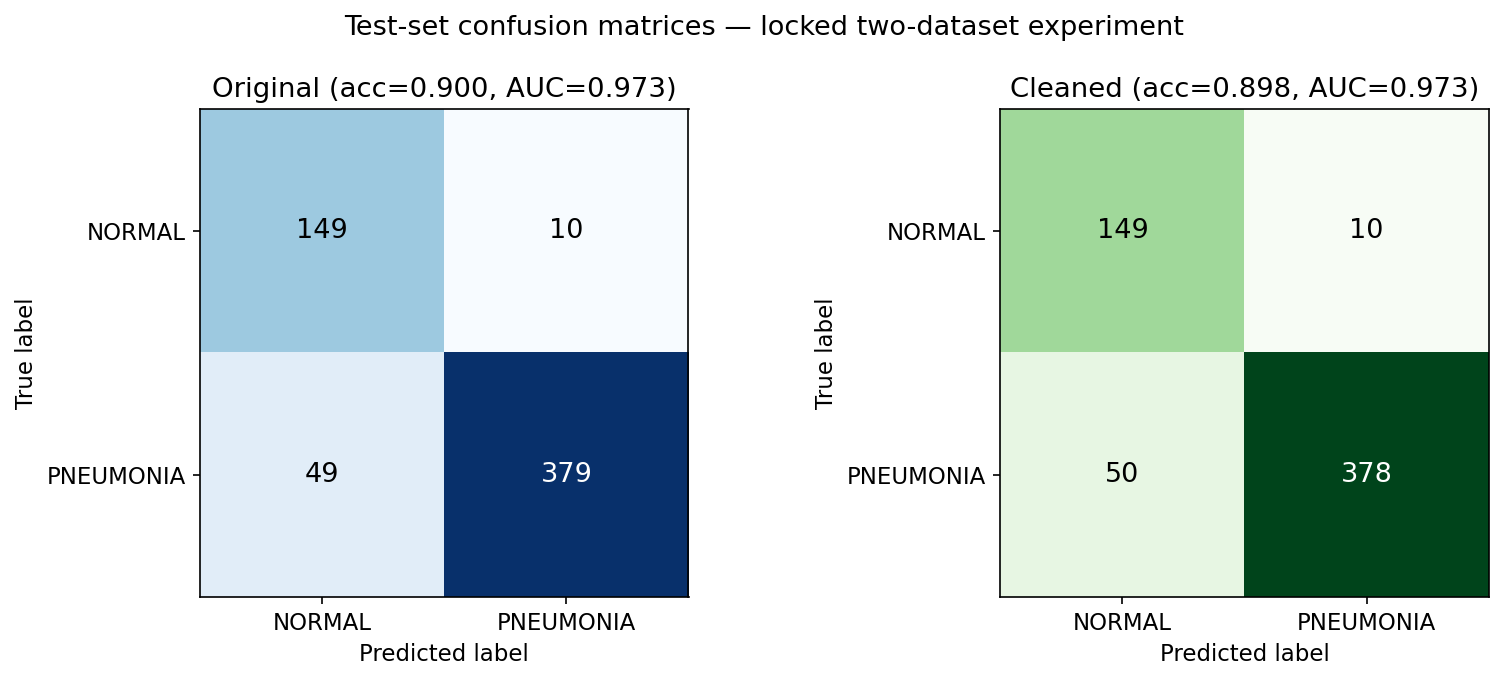
\includegraphics[width=\linewidth]{figs/fig_confusion.png}
\caption{Test-set confusion matrices for the model trained on the original
images (left) and on the cleaned images (right).}
\label{fig:confusion}
\end{figure}

\begin{figure}[t]
\centering
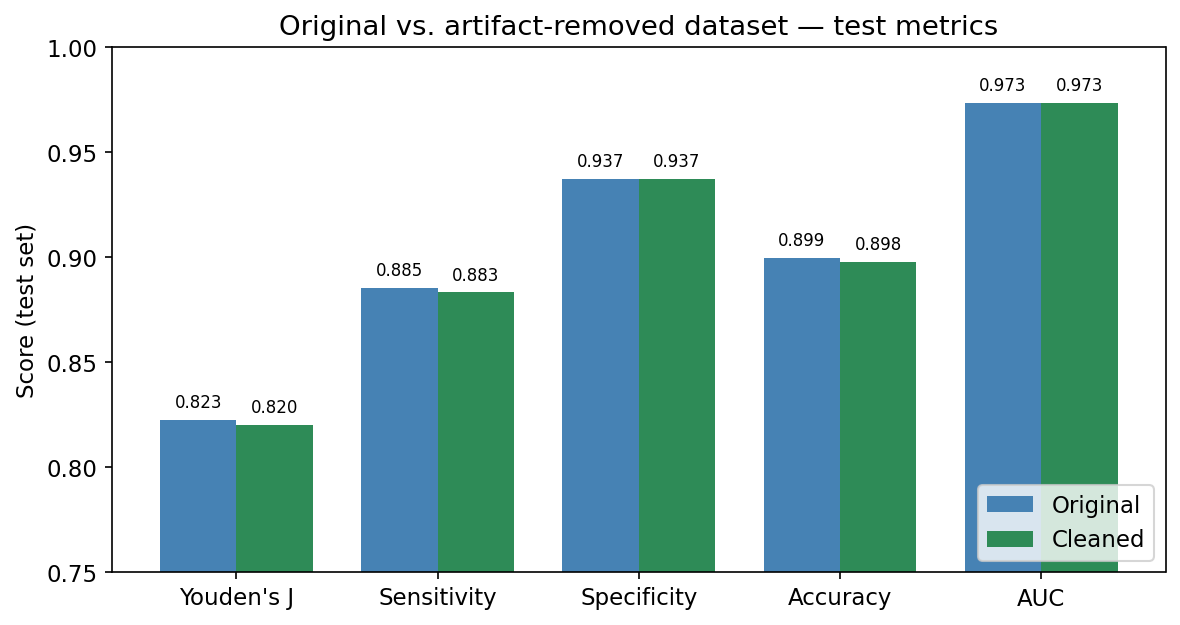
\includegraphics[width=\linewidth]{figs/fig_comparison.png}
\caption{Test metrics for the original and cleaned datasets. The bars are
visually indistinguishable across all five metrics.}
\label{fig:comparison}
\end{figure}

% =====================================================================
\section{Conclusion}
\label{sec:conclusion}
Returning to \textbf{Q1} (Section~\ref{sec:rq}): for this dataset and
architecture, removing non-anatomical artifacts did \emph{not} improve pneumonia
classification. Every test metric moved by less than $0.25$ percentage points and
all changes were slightly negative (Table~\ref{tab:results}, Section
\ref{sec:findings}) --- well within the run-to-run noise we would expect from a
single split. We therefore find no evidence that the baseline model was relying on
the orientation markers; its decisions appear to be driven by the lung fields,
not the burned-in text. In the language of Section~\ref{sec:intro}, the feared
shortcut \cite{geirhos2020shortcut,degrave2021shortcut} does not materially affect
performance here, most likely because the weighted sampler, augmentation and the
markers' position outside the lungs already limit their influence.

On the supporting questions, the OpenCV-plus-inpainting detector (Q1.1) removed
markers reliably and cheaply without harming anatomy
(Figure~\ref{fig:cleaning}), and the weighted sampler (Q1.2) kept the comparison
fair by neutralising the class imbalance.

These conclusions carry clear limitations. We tested a single custom CNN on a
single re-split of one paediatric dataset, and our cleaning targets only bright
\emph{border} markers rather than performing full lung-field segmentation, so
residual non-anatomical content may remain. A negative result on one split is
also not proof of no effect. Future work should (i) repeat the locked experiment
across several seeds and report confidence intervals, (ii) replace marker removal
with a pretrained U-Net lung segmentation so the model sees only lung tissue, and
(iii) use Grad-CAM saliency maps to verify \emph{directly} where the network
looks. Such explainability evidence would complement the behavioural result
reported here.

% =====================================================================
\begin{thebibliography}{99}
\small
\bibitem{rajpurkar2017chexnet} P.~Rajpurkar et~al.,
``CheXNet: Radiologist-Level Pneumonia Detection on Chest X-Rays with Deep
Learning,'' \emph{arXiv:1711.05225}, 2017.

\bibitem{geirhos2020shortcut} R.~Geirhos et~al.,
``Shortcut Learning in Deep Neural Networks,'' \emph{Nature Machine
Intelligence}, vol.~2, pp.~665--673, 2020.

\bibitem{zech2018confound} J.~R.~Zech et~al.,
``Variable generalization performance of a deep learning model to detect
pneumonia in chest radiographs: A cross-sectional study,'' \emph{PLOS Medicine},
vol.~15, no.~11, e1002683, 2018.

\bibitem{degrave2021shortcut} A.~J.~DeGrave, J.~D.~Janizek, S.-I.~Lee,
``AI for radiographic COVID-19 detection selects shortcuts over signal,''
\emph{Nature Machine Intelligence}, vol.~3, pp.~610--619, 2021.

\bibitem{nunamaker1990} J.~F.~Nunamaker~Jr., M.~Chen, T.~D.~M.~Purdin,
``Systems Development in Information Systems Research,'' \emph{Journal of
Management Information Systems}, vol.~7, no.~3, pp.~89--106, 1990.

\bibitem{kermany2018} D.~S.~Kermany et~al.,
``Identifying Medical Diagnoses and Treatable Diseases by Image-Based Deep
Learning,'' \emph{Cell}, vol.~172, no.~5, pp.~1122--1131, 2018.

\bibitem{kagglecxr} P.~Mooney,
``Chest X-Ray Images (Pneumonia),'' Kaggle dataset, 2018.
\url{https://www.kaggle.com/datasets/paultimothymooney/chest-xray-pneumonia}.

\bibitem{he2016resnet} K.~He, X.~Zhang, S.~Ren, J.~Sun,
``Deep Residual Learning for Image Recognition,'' \emph{CVPR}, 2016.

\bibitem{shorten2019augment} C.~Shorten, T.~M.~Khoshgoftaar,
``A Survey on Image Data Augmentation for Deep Learning,'' \emph{Journal of Big
Data}, vol.~6, no.~60, 2019.

\bibitem{he2009imbalanced} H.~He, E.~A.~Garcia,
``Learning from Imbalanced Data,'' \emph{IEEE Transactions on Knowledge and Data
Engineering}, vol.~21, no.~9, pp.~1263--1284, 2009.

\bibitem{krawczyk2016imbalanced} B.~Krawczyk,
``Learning from imbalanced data: open challenges and future directions,''
\emph{Progress in Artificial Intelligence}, vol.~5, pp.~221--232, 2016.

\bibitem{ioffe2015batchnorm} S.~Ioffe, C.~Szegedy,
``Batch Normalization: Accelerating Deep Network Training by Reducing Internal
Covariate Shift,'' \emph{ICML}, 2015.

\bibitem{srivastava2014dropout} N.~Srivastava et~al.,
``Dropout: A Simple Way to Prevent Neural Networks from Overfitting,''
\emph{Journal of Machine Learning Research}, vol.~15, pp.~1929--1958, 2014.

\bibitem{lecun1998gradient} Y.~LeCun, L.~Bottou, Y.~Bengio, P.~Haffner,
``Gradient-Based Learning Applied to Document Recognition,'' \emph{Proceedings of
the IEEE}, vol.~86, no.~11, pp.~2278--2324, 1998.

\bibitem{krizhevsky2012imagenet} A.~Krizhevsky, I.~Sutskever, G.~E.~Hinton,
``ImageNet Classification with Deep Convolutional Neural Networks,''
\emph{NeurIPS}, 2012.

\bibitem{bradski2000opencv} G.~Bradski,
``The OpenCV Library,'' \emph{Dr.\ Dobb's Journal of Software Tools}, 2000.

\bibitem{telea2004inpaint} A.~Telea,
``An Image Inpainting Technique Based on the Fast Marching Method,''
\emph{Journal of Graphics Tools}, vol.~9, no.~1, pp.~23--34, 2004.

\bibitem{bergstra2012random} J.~Bergstra, Y.~Bengio,
``Random Search for Hyper-Parameter Optimization,'' \emph{Journal of Machine
Learning Research}, vol.~13, pp.~281--305, 2012.

\bibitem{youden1950} W.~J.~Youden,
``Index for rating diagnostic tests,'' \emph{Cancer}, vol.~3, no.~1,
pp.~32--35, 1950.
\end{thebibliography}

\end{document}
